% Original experimental story. Every plotted point is synthetic teaching data.
\documentclass[10pt,aspectratio=169]{beamer}
\usetheme[progressbar=frametitle]{metropolis}
\usepackage{amsmath,booktabs,pgfplots}
\pgfplotsset{compat=1.18}
\title{When should a classifier abstain?}
\subtitle{An experiment before an architecture diagram}
\author{Machine learning reading group}
\date{}
\begin{document}
\maketitle
\section{Decision}
\begin{frame}{Would you deploy either model?}
\begin{table}\centering
\begin{tabular}{lrr}\toprule
Model & Accuracy & Predictions returned\\\midrule
A & 92\% & 100\%\\
B & 97\% & 60\%\\\bottomrule
\end{tabular}
\caption{Illustrative values, not benchmark results.}
\end{table}
\pause
\alert{The denominator changed.} Accuracy alone cannot price unanswered cases.
\note{Ask whether the deployment has a human review path. Do not rank the models before discussing the cost of rejection.}
\end{frame}
\begin{frame}{Make the selection rule explicit}
Let $p_\theta(y\mid x)$ be class probabilities and $s(x)=\max_y p_\theta(y\mid x)$.
\begin{align*}
 g_\tau(x)&=\mathbf{1}\{s(x)\geq\tau\},\\
 C(\tau)&=\mathbb{E}[g_\tau(X)],\\
 R(\tau)&=\frac{\mathbb{E}[\ell(f(X),Y)g_\tau(X)]}{C(\tau)},\qquad C(\tau)>0.
\end{align*}
Coverage $C$ and selective risk $R$ answer different questions.\footnote{The expectation is over the evaluation population; empirical estimates use its held-out sample.}
\end{frame}
\section{Experiment}
\begin{frame}{An operating point is a policy choice}
\begin{columns}[T,onlytextwidth]
\begin{column}{.62\textwidth}
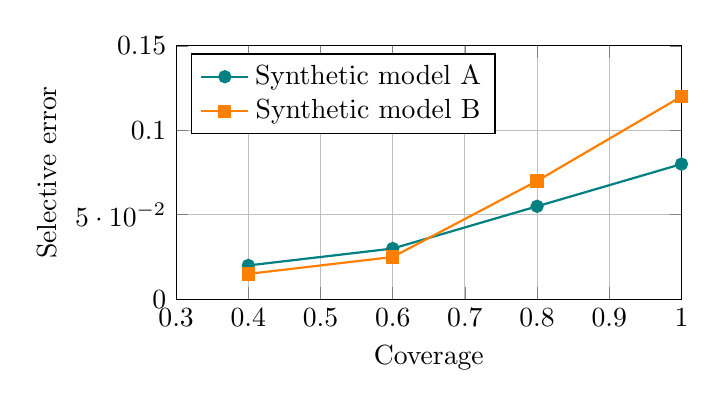
\begin{tikzpicture}\begin{axis}[width=8cm,height=4.8cm,xmin=.3,xmax=1,ymin=0,ymax=.15,
 xlabel={Coverage},ylabel={Selective error},legend pos=north west,grid=major]
\addplot[mark=*,thick,teal] coordinates {(.4,.02) (.6,.03) (.8,.055) (1,.08)};
\addlegendentry{Synthetic model A}
\addplot[mark=square*,thick,orange] coordinates {(.4,.015) (.6,.025) (.8,.07) (1,.12)};
\addlegendentry{Synthetic model B}
\end{axis}\end{tikzpicture}
\end{column}
\begin{column}{.34\textwidth}
At high coverage, the ordering reverses.
\medskip
Choose the acceptable region \emph{before} tuning the threshold on held-out data.
\end{column}
\end{columns}
\end{frame}
\begin{frame}{The evaluation split is part of the method}
\begin{enumerate}[<+->]
\item Fit model parameters on training data.
\item Choose a threshold using validation data and a stated cost.
\item Freeze both choices.
\item Estimate coverage and error on untouched test data.
\end{enumerate}
\begin{alertblock}{Leakage check}
Trying many thresholds on the test set turns it into another validation set.
\end{alertblock}
\end{frame}
\begin{frame}{Rejection can hide a subgroup failure}
\begin{overprint}
\onslide<1>
\begin{block}{Aggregate report}
The system returns predictions for 80\% of cases with low error.
\end{block}
\onslide<2>
\begin{alertblock}{Disaggregated report}
One subgroup receives only 30\% coverage. A low aggregate error did not reveal who was rejected.
\end{alertblock}
\end{overprint}
\medskip
Report coverage, risk, and sample size together for each prespecified slice.
\end{frame}
\section{Interpretation}
\begin{frame}{Confidence and calibration are different claims}
\begin{columns}[T]
\begin{column}{.48\textwidth}\begin{block}{Confidence score}
A scalar used to rank or select predictions. Large values do not by themselves prove reliability.
\end{block}\end{column}
\begin{column}{.48\textwidth}\begin{exampleblock}{Calibration question}
Among comparable predictions assigned probability $q$, is the event frequency close to $q$?
\end{exampleblock}\end{column}
\end{columns}
A rejection rule may change the population on which calibration is assessed.
\end{frame}
\begin{frame}{Design the next experiment}
\begin{itemize}
\item Compare a confidence threshold with a separate selection model.
\item Prespecify rejection cost and a maximum review volume.
\item Evaluate a shifted population as a separate condition.
\end{itemize}
\bigskip
\textbf{Deliverable:} one risk--coverage curve, one subgroup table, and a paragraph stating what remains unidentified.
\end{frame}
\appendix
\begin{frame}{Reading and reproducibility boundary}
\small
\begin{thebibliography}{9}
\bibitem{selective} \emph{Calibrated Selective Classification} (2022).
\href{https://arxiv.org/abs/2208.12084}{Research paper}.
\end{thebibliography}
This deck uses original definitions-based examples and invented data. Its curves are not a reproduction of the paper's experiments and imply no empirical ranking of real models.
\end{frame}
\end{document}
